\section{Zadání}
Nasimulujte spektrální vlastnosti vláknových mřížek. Odrazivosti jednotlivých typů mřížek
vložte do jednoho grafu a porovnejte výsledné vlastnosti. Parametry simulovaných mřížek
jsou následující: 
\begin{table}[h]
    \centering
    \small
    \begin{tabular}{|p{2.5cm}|p{3.9cm}|p{6cm}|p{3.9cm}|}
        \hline
        \textbf{Typ mřížky} & \textbf{Homogenní mřížka} & \textbf{Apodizovaná mřížka (bez kompenzace, s kompenzací $n_{eff}$)} & \textbf{Chirpovaná mřížka} \\ \hline
        Délka [mm] & 30 & 30 & 10 \\ \hline
        $\Delta n$ & 3E-5 & 6E-5 & 5E-4 \\ \hline
        Chirp [nm/mm] & 0 & 0 & 0.2 \\ \hline
        Profil apodizace & Homogenní (bez apodizace) & Gaussovský (bez kompenzace, s kompenzací) & Homogenní (bez apodizace) \\ \hline
        Spektrum [nm] & 1549-1551 & 1549-1551 & 1544-1556 \\ \hline
    \end{tabular}
    \caption{Porovnání mřížek}
    \normalsize
\end{table}

Pro všechny mřížky zvolte parametry vlákna: \(nc = 1.4488\), \(ncl = 1.44402\), \(d = 9.6 [\mu m]\). 
Všechny simulace provádějte pro rezonanční vlnovou délku \(1550 [nm]\). 
Počet sekcí volte tak, aby vycházela přibližně 1 sekce na \(50 [\mu m]\) délky mřížky.
Dále zjistěte, jak následující parametry mění výsledné spektrální vlastnosti mřížky: délka, změna indexu lomu \(\delta n\), tvar periody, hustota vzorkování.
Z grafů odečtěte šířku odraženého pásma při poklesu o \(3 [dB]\), maximální odrazivost v \% a potlačení postranních pásem oproti hlavnímu maximu v \(dB\). 
Pro lineárně chirpovanou mřížku určete také směrnici grupového zpoždění. 

\newpage

\section{Simulace}

\begin{figure}[h!]
    \centering
    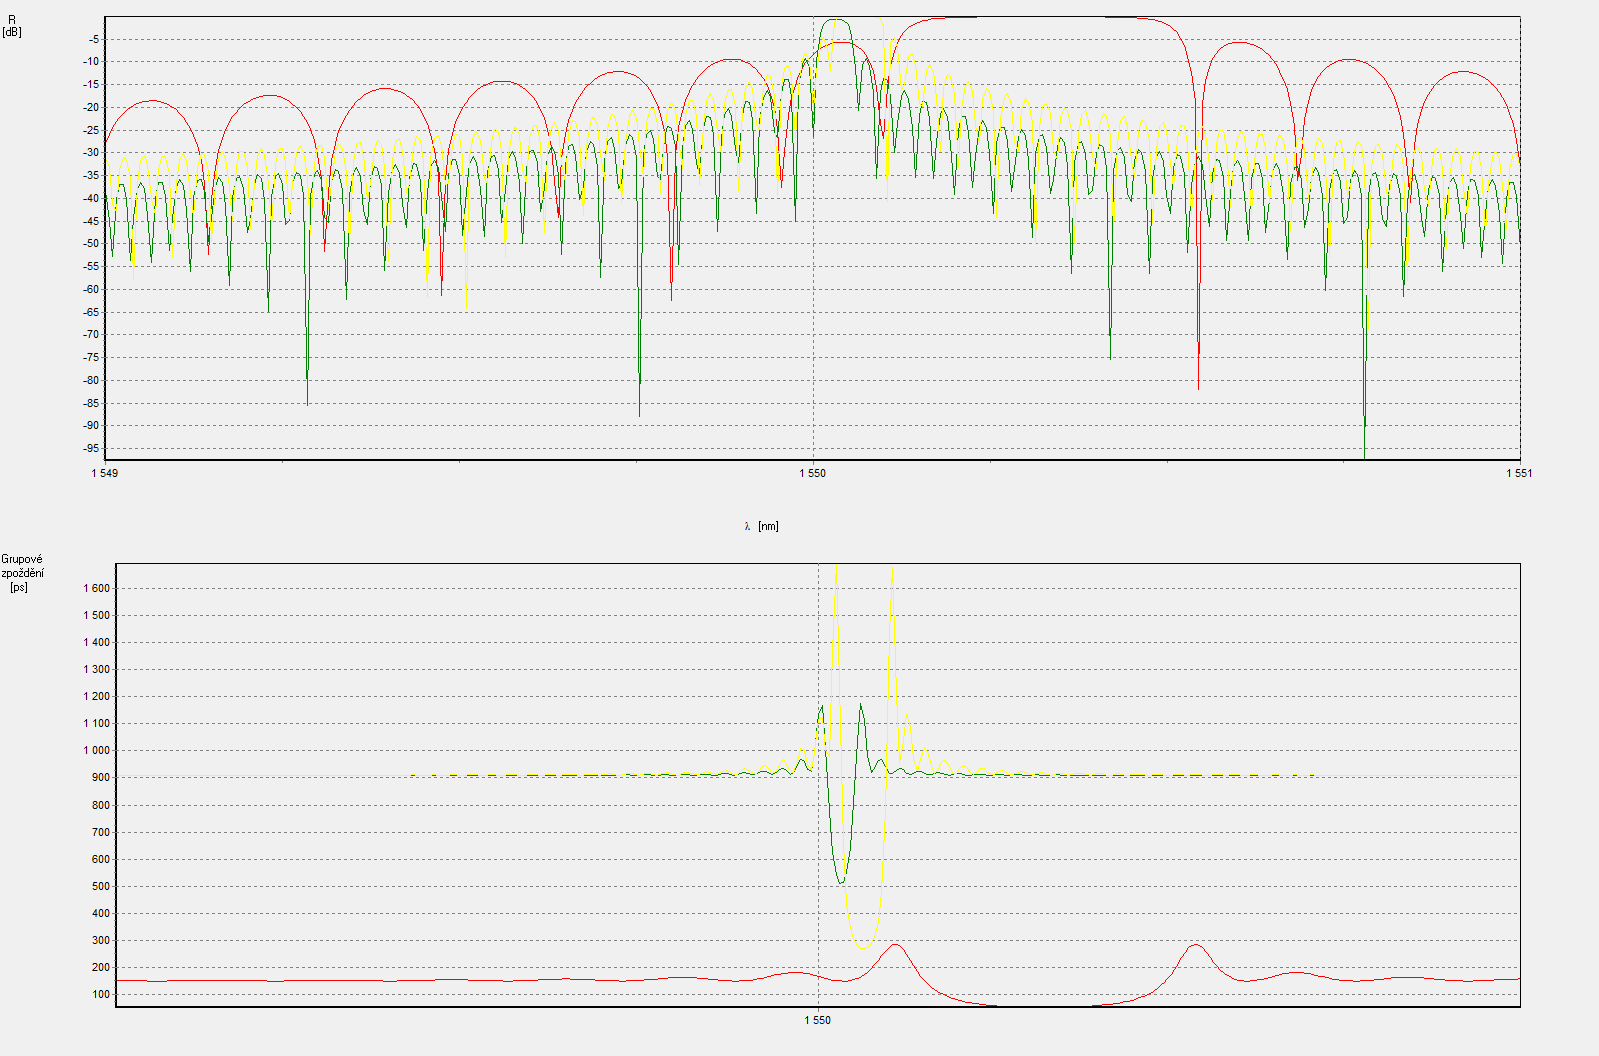
\includegraphics[width=\textwidth]{text/img/simulace-1.png}
    \caption{\label{fig:simulace} simulace}
\end{figure}

